\begin{proof}[证明]

  设$uv$为三次图$G$的一座桥,则$G-uv$包含两个支,其中一个支包含顶点$u$,另一个顶点包含顶点$v$。
  在包含顶点$u$的支中,至少含有一个顶点度为3,因此至少包含$4$个顶点。此时,如果该支中只包含$4$个顶点,则它们的度依次为$2,3,3,3$,这是不可能的(任意一个图中度为奇数的顶点的个数必为偶数)。因此,该支中至少包含$5$个顶点。同理,包含$v$的支至少包含$5$个顶点,如下图所示,结论得证。
  
     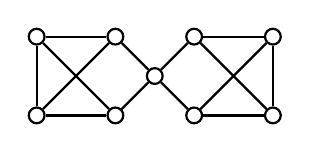
\begin{tikzpicture}[auto,
    specification/.style ={circle, draw, thick, inner sep = 0pt, minimum size=2mm}]
   \node[specification] (A)  at (0,0.5)  {};
   \node[specification] (B)  at (0,-0.5)  {};
   \node[specification] (C)  at (1,0.5)  {};
   \node[specification] (D) at (1,-0.5)  {};
   \node[specification] (E)  at (1.5,0)  {};
   \node[specification] (F)  at (2,0.5)  {};
   \node[specification] (G)  at (2,-0.5)  {};
   \node[specification] (H)  at (3,0.5)  {};
   \node[specification] (I)  at (3,-0.5)  {};
   
   \draw[thick] (A) to  (B);
   \draw[thick] (B) to  (C);
   \draw[thick] (A) to  (D);
   \draw[thick] (A) to  (C);
   \draw[thick] (B) to  (D);

   \draw[thick] (C) to  (E);
   \draw[thick] (D) to  (E);
   
   \draw[thick] (E) to  (F);
   \draw[thick] (E) to  (G);
   \draw[thick] (G) to  (H);
   \draw[thick] (H) to  (I);
   \draw[thick] (I) to  (F);
   \draw[thick] (F) to  (H);
   \draw[thick] (G) to  (I);
 \end{tikzpicture}                     

\end{proof}
